\documentclass[../main.tex]{subfiles}
\graphicspath{{\subfix{../images/}}}
\begin{document}


\subsection{Předpodmiňování metody složených gradientů}
Aplikací CG (konjugovaných gradientů) na předpodmíněnou soustavu 
\begin{equation*}
\mathbb{L}^{-1}\mathbb{A}\mathbb{L}^{-1^T} y = \mathbb{L}^{-1}b, \mathbb{L}^{-1^T}y = x, \mathbb{M} = \mathbb{L}\mathbb{L}^T
\end{equation*}

Lze odvodit algoritmus PCG \todo{dopln jmeno}
\begin{enumerate}
    \item vstup: $\mathbb{A}\in\mathbb{R}^{n,n}$ SPD,$x_0\in\mathbb{R}^n$ libovolný.
    \item $r_0 = b - \mathbb{A}x_0$
    \item vyřeš: $\mathbb{M}z_0 = r_0$, $z_0$ je předpodmíněné reziduum
    \item $d_0 = z_0$
    \item for $i=0,1\dots$ až je aproximace dost přesná \begin{enumerate}
        \item $\alpha_i = \frac{<r_i, z_i>}{<d_i, \mathbb{A}d_i>}$
        \item $x_{i+1} = x_i + \alpha_i d_i$
        \item $r_{i+1} = r_i - \alpha_i \mathbb{A} d_i$
        \item vyřeš $\mathbb{M}z_{i+1} = r_{i+1}$
        \item $\beta_i = \frac{<r_{i+1}, z_{i+1}>}{<r_i, z_i>}$
        \item $d_{i+1} = z_{i+1} + \beta_i d_i$
    \end{enumerate}
    \item end for 
\end{enumerate}

\begin{remark}
    Při porovnání s normálními konjugovanými gradienty si všimněme rozdílu pouze v pár krocích
\end{remark}

\subsection{Rychlost konvergence PCG}

O konjugovaných gradientech pro konvergenci víme následující \begin{equation*}
    ||x_n -x ||_\mathbb{A} \leq 2 \left( \frac{\sqrt{\varkappa(\mathbb{A})}-1}{\sqrt{\varkappa(\mathbb{A})}+1} \right)^n ||x_0 -x||_\mathbb{A}
\end{equation*}
předpodmínění $\mathbb{M} = \mathbb{L} \mathbb{L}^T$ bude účinné, pokud $\varkappa(\mathbb{L}^{-1}\mathbb{A}\mathbb{L}^{-1^T}) << \varkappa(\mathbb{A})$

\matA je SPD s vlastními čísly: $0 < \lambda_1 \leq \lambda_2 \leq \dots \leq \lambda_n$.

Poté $\varkappa(\mathbb{A}) = \frac{\lambda_n}{\lambda_1}$. Toto je dobré, pokud vlastní čísla $\mathbb{L}^{-1}\mathbb{A}\mathbb{L}^{-1^T}$ tvoří malý shluk daleko od 0.



\subsection{Testovací případ}
Vezměme matici \matA která pochází z diskretizace Poissonovy rovnice $u''(x)=f(x), u(0)=u(1)=0$ metodou sítí, $h = \frac{1}{n+1}$.\\

Například $A_3 = \begin{pmatrix}
    2 & -1 & 0\\
    -1 & 2 & -1 \\
    0 & -1 & 2
\end{pmatrix}$

Platí následující:\\
\matA je SPD 
\begin{equation*}
    k\in\hat{n}: \lambda_k = 4 \sin^2 \frac{k\pi}{2(n+1)}, v_k = \left( \sin \frac{i k \pi}{n+1}\right)^n_{i+1}
\end{equation*}
    
\subsubsection{Metoda prosté iterace}
$\mathbb{M} = \mathbb{I}$
\begin{equation*}
    \varrho(\mathbb{I} - \mathbb{A}) = \max_{k\in\hat{n}} |1-\lambda_k| = \max_{k\in\hat{n}} |1 - 4 \sin^2 \frac{k\pi}{2(n+1)}|
    = \max \left\{ |1-\lambda_1|, 1 - \lambda_n  \right\} = \max \left\{ < 1, \approx 3  \right\} \approx 3
\end{equation*}
Metoda prosté iterace NEkonverguje!, je nutno předpodmiňovat.



\subsubsection{Richardson}
$\mathbb{M} = \frac{1}{\omega} \mathbb{I}, \omega\in\mathbb{R}$


\begin{equation*}
    \varrho(\mathbb{I} - \omega \mathbb{A}) = \max_{k\in\hat{n}} |1-\omega\lambda_k| = \max |1 - 4\omega \sin^2 \frac{k\pi}{2(n+1)}|
\end{equation*}

Z toho plyne, že $\omega$ je třeba volit tak aby $1 - 4\omega \sin^2 \frac{k\pi}{2(n+1)} \in (-1,1)$, proto\begin{equation*}
    1 - 4\omega \sin^2 \frac{k\pi}{2(n+1)} > 1 - 4\omega \sin^2 \frac{\pi}{2} > -1
\end{equation*}
Z toho plyne, že stačí volit $\omega \leq \frac{1}{2}$

Pro konvergenci Richardsonovy metody je nutná a postačující podmínka, že $\omega\in(0;\frac{1}{2}\rangle$

\begin{multline*}
    \varrho(\mathbb{I} - \omega \mathbb{A}) = \max \left\{ |1-\omega\lambda_1|, 1 - \omega\lambda_n  \right\} =\\
    \max \left\{ |1-4\omega \sin^2 \frac{\pi}{2(n+1)}|, 1 - 4\omega \sin^2 \frac{n\pi}{2(n+1)}  \right\} =\\
    \max \left\{ 1-O(h^2), 1 - 4\omega \cos^2 \frac{\pi}{2(n+1)}  \right\}
\end{multline*}

Poslední rovnost plyne z \begin{equation*}
    \sin\frac{n\pi}{2(n+1)} = \sin \left(\frac{\pi}{2} - \frac{\pi}{2(n+1)}\right) = \cos \frac{\pi}{2(n+1)}
\end{equation*}

Pro $\omega = \frac{1}{2}$ je maximum ze 2 stejných čísel. Z toho\begin{equation*}
    \varrho(\mathbb{I} - \omega \mathbb{A}) = 1 - O(h^2)
\end{equation*}
Pro $h \rightarrow 0+$ se konvergence zastavuje.


\subsubsection{Jacobi}

$\mathbb{M} = \mathbb{D} = diag(\mathbb{A}) \implies$ Richardson s $\omega = \frac{1}{2}$

\begin{multline*}
    \varrho(\mathbb{I} - \mathbb{D}^{-1}\mathbb{A}) = \max \left\{  |1-\frac{1}{2}\lambda_1|, 1 - \frac{1}{2}\lambda_n \right\} =\\
    \max \left\{ |1-2 \sin^2 \frac{\pi}{2(n+1)}|, 1 - 2 \sin^2 \frac{n\pi}{2(n+1)}  \right\} =\\ 1 - 2 \sin^2 \frac{\pi}{2(n+1)}
    = 1 - 2 \sin^2 \frac{\pi h}{2} = 1 - O(h^2)
\end{multline*}

\subsubsection{Gauss-Seidel a SOR(w)}
\matA je dvoucyklická a shodně uspořádaná. Proto lze použít teorii z numerické matematiky. O rychlosti konvergence rozhoduje
$\varrho(\mathbb{I} - (\frac{1}{\omega}\mathbb{D} -\mathbb{L})^-1 )\mathbb{A}$, kde označme $G_{SOR} \coloneq \mathbb{I} - (\frac{1}{\omega}\mathbb{D} -\mathbb{L})^-1 )\mathbb{A}$.
Vlastní čísla $\lambda\in\sigma(G_{SOR})$ a $\mu \in \sigma(G_{Jacobi})$ jsou svázaná rovnicí 
$(\lambda + \omega -1 )^2 = \omega^2 \mu^2 \lambda$.

Gauss-Seidel: $\omega = 1: \lambda = \mu^2$
\begin{equation*}
    \varrho(\mathbb{I} - (\mathbb{D}- \mathbb{L})^{-1} \mathbb{A}) = \varrho(\mathbb{I} - \mathbb{D}^{-1} \mathbb{A})^2 =
    (1 - 2 \sin^2 \frac{\pi}{2(n+1)}) = 1 - 4 \sin^2 \frac{\pi}{2(n+1)} + 4 \sin^4 \frac{\pi}{2(n+1)} = 1 - O(h^2)
\end{equation*}

Všimněme si že i přesto, že GS konverguje rychleji než Jacobi tak se také konvergence zastavuje.

% SOR(w) : $\omega \in (0,2)$
% 



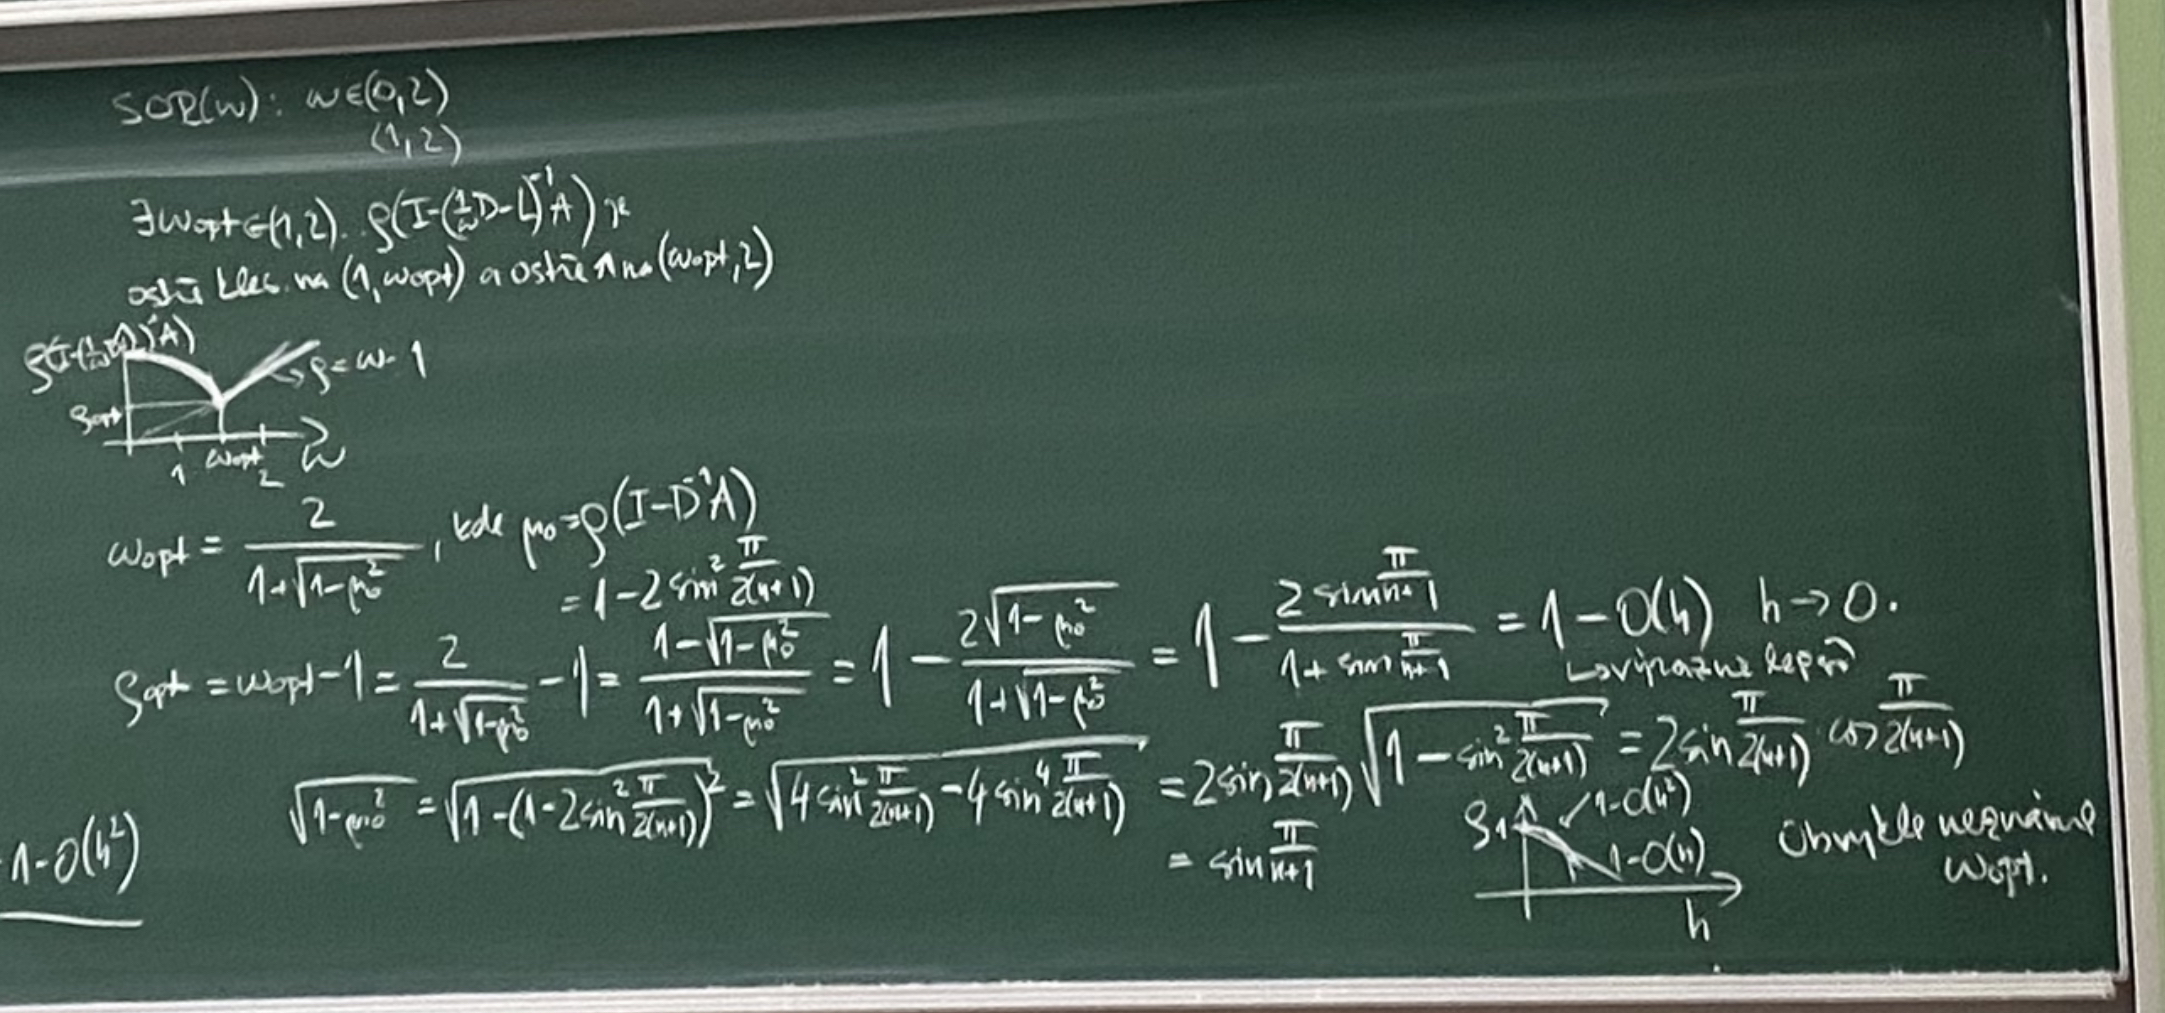
\includegraphics[width=0.9\linewidth]{images/23-11-SOR.jpg}





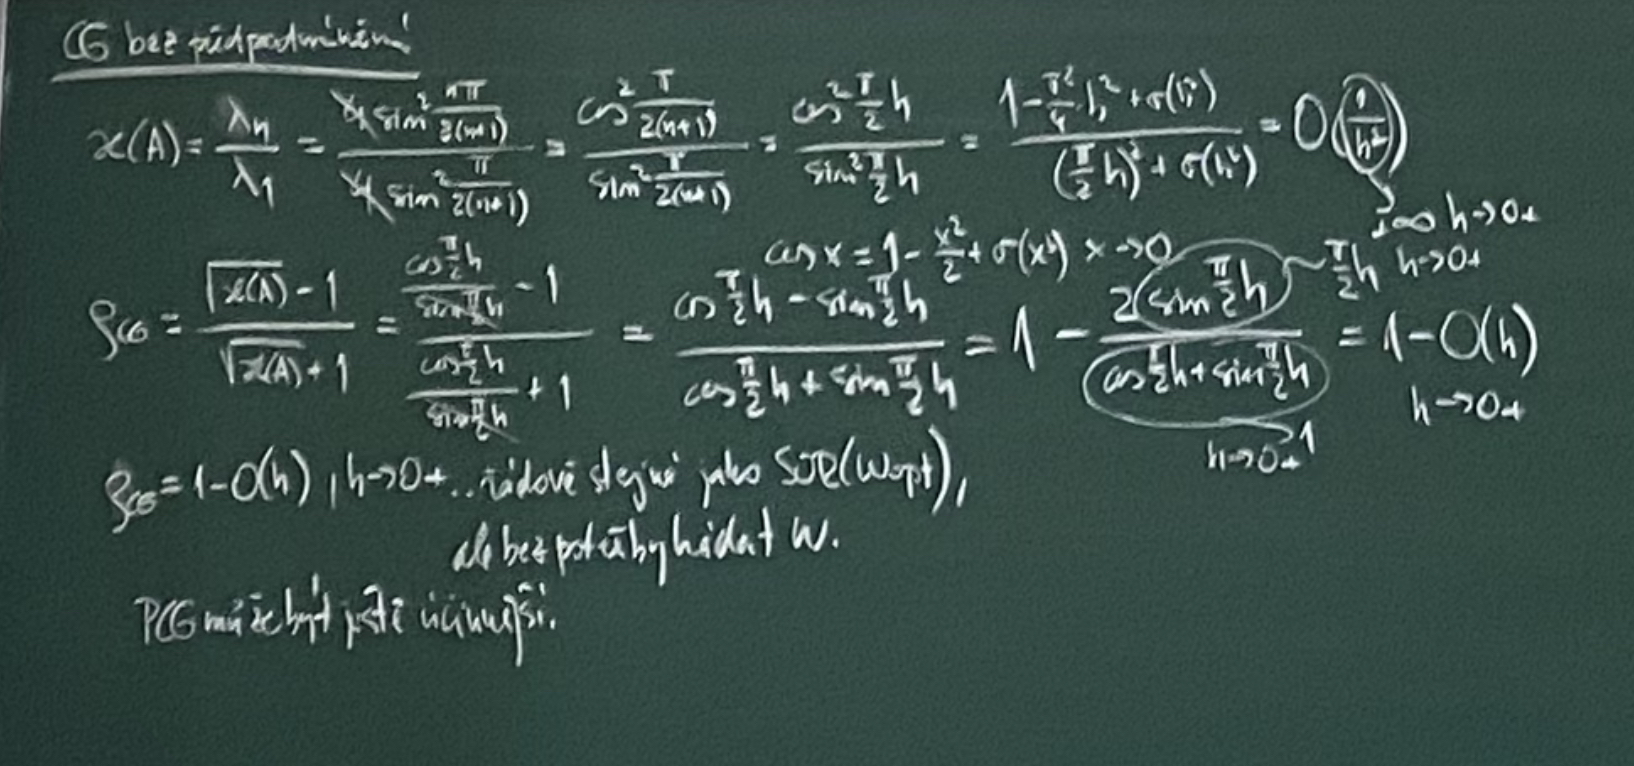
\includegraphics[width=0.9\linewidth]{images/23-11-CG.jpg}






\end{document}